\chapter{Evaluation\label{chap:evaluation}}
  This chapter will detail the evaluation metrics, how they were tested and what the results of the evaluation were. Two (or three) sets of evaluations were carried out making use of six debates from our corpus \cite{walker2012corpus}: abortion, creation, gay rights, the existence of god, gun ownership and healthcare.

  \section{Research Questions}
    We wanted to evaluate our tool as a tool for automated summarization. The result of a final analysis was a summary comprising of point extracts for a given debate, by assessing the quality of this we also evaluate the precursor analysis. The following research questions were set:

    \begin{itemize}
      \item{Are our summaries more readable and informative than those produced by existing tools?}
      \item{Does introducing summary sections with an explanation improve readability?}
      \item{What is the level of agreement between our extract selection module and humans given the same task?}
      \item{TBD: Which sections of generated summaries are most useful to readers?}
    \end{itemize}

    To address these questions we compared different versions of our summaries against equal-length summaries generated by an implementation of \cite{nenkova2006compositional} (`stock summaries'). We also gathered scores for groups of extracts and compared summaries generated with randomly selected extracts against one based on our bigram model for selection.

  \section{Design}
    In response to the our research questions we set the following null hypotheses for the evaluation:

    \begin{itemize}
      \item{The readability and informativeness of our summaries do not improve on those of existing tools. (\textbf{H1})}
      \item{Explanations introducing summary sections does not improve readability. (\textbf{H2})}
      \item{Our means of selecting extracts is not better than random selection. (\textbf{H3})}
      \item{\textcolor{red}{TBD: All summary sections are equally useful to readers. (\textbf{H4})}}
    \end{itemize}

    To test these hypotheses we prepared three comparative studies. These are described in the following sections.

    \tocless\subsection{Summary Styles}
      In the upcoming sections, reference is made to a range of summary styles.
      \begin{itemize}
        \item{\textbf{Stock}: A summary generated using an implementation of \cite{nenkova2006compositional}, used as a benchmark for summaries generated by our tool. There is no structure to these summaries.}
        \item{\textbf{Plain}: This is a collection of point extracts in the same styles as the stock summaries. The order of extracts is the same as it would be if the summary had sections annotated. This presentation is designed to be as close as possible to the stock summary presentation.}
        \item{\textbf{Layout}: A summary that has explanatory text that introduces sections. The extracts are the same as those in the plain summary.}
        \item{\textbf{Formatted}: A layout summary with explanation keywords in bold and topic words in green.}
      \end{itemize}

      Participants for Study 1 and 2 were recruited using Amazon Mechanical Turk. \textcolor{red}{In the third study\dots}

    \tocless\subsection{Study 1: Summary Comparison}
      In order to address \textbf{H1} and \textbf{H2} we designed a questionnaire that compared various summary styles against equal-length stock summaries. Each questionnaire was made up of three sections.

      The first section compared a plain summary against a stock summary, on the same topic. Users were instructed to read both summaries and rate them relatively on the following criteria: `Content Interest / Informativeness', `Readability', `Punctuation \& Presentation' and `Organization'. Finally they they were asked to give an overall rating and justify their response. The next section asked the same questions but instead compared a layout summary against a stock one. Layout summaries are longer because of the explanatory text, the stock summary was the same length as the layout summary and was longer than the stock summary used in the first section. The final section compared a layout summary with a formatted one. The layout summary is reused from the second section, the formatted summary is also the same content (only different formatting). There was only an overall rating and justification for the comparison in this section.

      There were six versions of the questionnaire setup in a Latin square to cover all six topics. Section 1 had a different topic from sections 2 so as to not repeat summary content. Section 3 addresses the question of formatting only and has the same content as the layout summary in section 2 to make the task faster.

      Responses from the first section that compare our plain summary against a stock one can be used in addressing \textbf{H1}. The difference in the responses gathered in section 2 will allow us to address \textbf{H2}. Section 3 extends on this, testing if the formatting is a useful addition to the layout summary.

    \tocless\subsection{Study 2: Extract Comparison}
      To investigate the performance of the tool in greater depth we ran a further study testing the quality of our extract selection mechanism. Responses from this questionnaire addressed \textbf{H3}.

      The task given to participants had two sections. First were a series of extracts for a number of point patterns, participants were asked to rate extracts accounting for their succinctness and the extent to which they made sense. This was the closest we could make the task for participants to that of the tool. The following section, similar to the first study compared two summaries. Both summaries were of the formatted style however their content differed. The extracts in one summary were selected using the bigram model, the extracts in the other were selected at random. Participants were asked to give these a relative rating and justify their response. Responses for these two tasks were both intended to address \textbf{H3}.

    \tocless\subsection{\textcolor{red}{TBD: Study 3: Section Comparison}}

  \section{Results}
    \subsection{Study 1: Summary Comparison}
      The results of the summary comparison showed a strong preference for summaries based on points based extraction. When comparing the plain and stock summaries, our plain summaries were marked as better or much better by 69\% of participants. Plain summaries, lacking any kind of layout, was still scored better or much better by 57\% of participants.

      When comparing layout summaries against equal length stock summaries participant preference only became clearer. 89\% of participants rated layout as better or much better than stock. Organization saw the greatest change, with a 30\% increase in favor of layout summaries. The average increase across all factors was 19\%. The ratio of `better' to `much better' also shifted, `much better' ratings increased by 15\% while `better' ones decreased by 5\%.

      There was also variation between summaries of different discussions. The gay rights layout summary saw an increase of 45\% in better/much better scores while the guns layout summary saw no improvement. When comparing plain and stock summaries on guns and healthcare all participants rated plain as being the same or better. When comparing the healthcare layout and stock summaries all participants marked the layout summary as being much more readable. The plain vs stock creation summary was the most divided, 42\% of responses were marked as same or stock better.

      Despite the points used in the layout and plain summaries being the same, the `Content' factor saw an increase of 14\% in better/much better scores. Punctuation was also saw a 13\% increase, despite also being the same.

      Regarding the results of the layout / formatted summary comparison, more than half of respondents preferred the formatted version of the summary. This is significantly lower than the improvements of layout vs stock (89\%) or even plain vs stock (69\%).

      These findings are based on the 55 responses from 6 different questionnaires giving 165 summary comparisons, the target population being people interested in online discussions.

      To test the significance of these results we use one-sided Sign test for matched pairs. Neutral responses were excluded, better \& much better responses were amalgamated. When comparing plain against stock, 38 successes in 45 trials, we found the probability for success is not equal with $p << 0.01$ (\textbf{H1}). Comparing layout and stock summaries, 49/53, we found that success is also not equal, $p << 0.01$. However, when comparing the layout and formatted summaries, 29/41, we found $p = 0.16$ and thus unsuitable to reject the null hypothesis at this level. These results are based on all responses across the different topics.

      (need to show that the layout improves on the plain vs stock, not sure how adjust my data to a Friedman Rank Sum Test)

      To conclude, the results show a preference for points based summaries. This can further be improved by introducing sections (if I can show statistical significance?). However we cannot say decisively that our formatted summaries improve on our layout versions.

    \subsection{Study 2: Extract Comparison}
      Our second study also gave a clear result. Extracts selected by our tool for display were scored above the user's mean score 74\% of the time. Selected extracts scored 3.94/5 on average while extracts not selected scored 3.11/5.

      (Results of a Mann-Whitney U test, or some other means of comparing the selected vs not extracts regarding the values from the likert scale scores. This is quite hard\dots)

      Currently results of a MWU test would read (where A is selected and B is not selected by the tool): The medians of Group A and Group B were 5 and 3, respectively. We ran a Mann-Whitney's U test to evaluate the difference in the responses of our 5-Likert scale question. We found a significant effect of Group (The mean ranks of Group A and Group B were 1026 and 767, respectively; U = *155681*, Z = *7.045*, p= 1.851 * 10\^-12, r = 0.0.17).

      \begin{figure}[h]
        \caption{\textcolor{red}{SAMPLE PLOT, machine z scores vs z scores of \textit{mean} human ratings}}
        \centering
        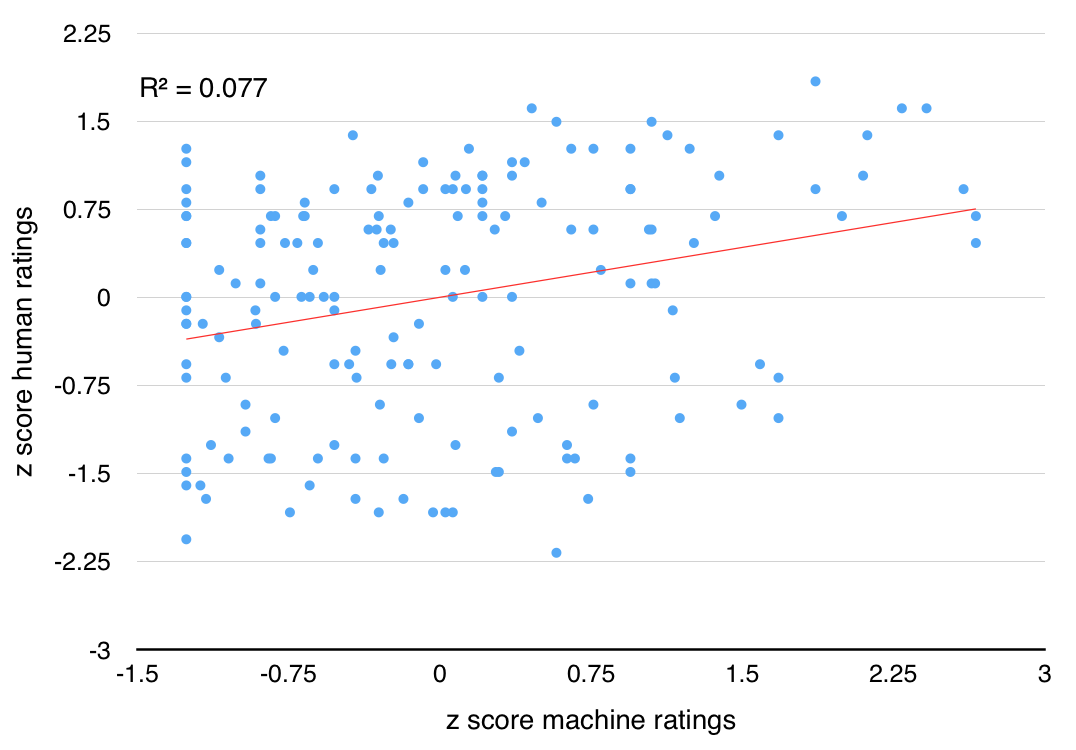
\includegraphics[width=0.8\textwidth]{extract_z_scores}
      \end{figure}

      Or the results can be presented like this:
      \begin{figure}[h]
        \caption{\textcolor{red}{group the human scores 1-5, then for each score plot the corresponding machine score in the box plot}}
        \centering
        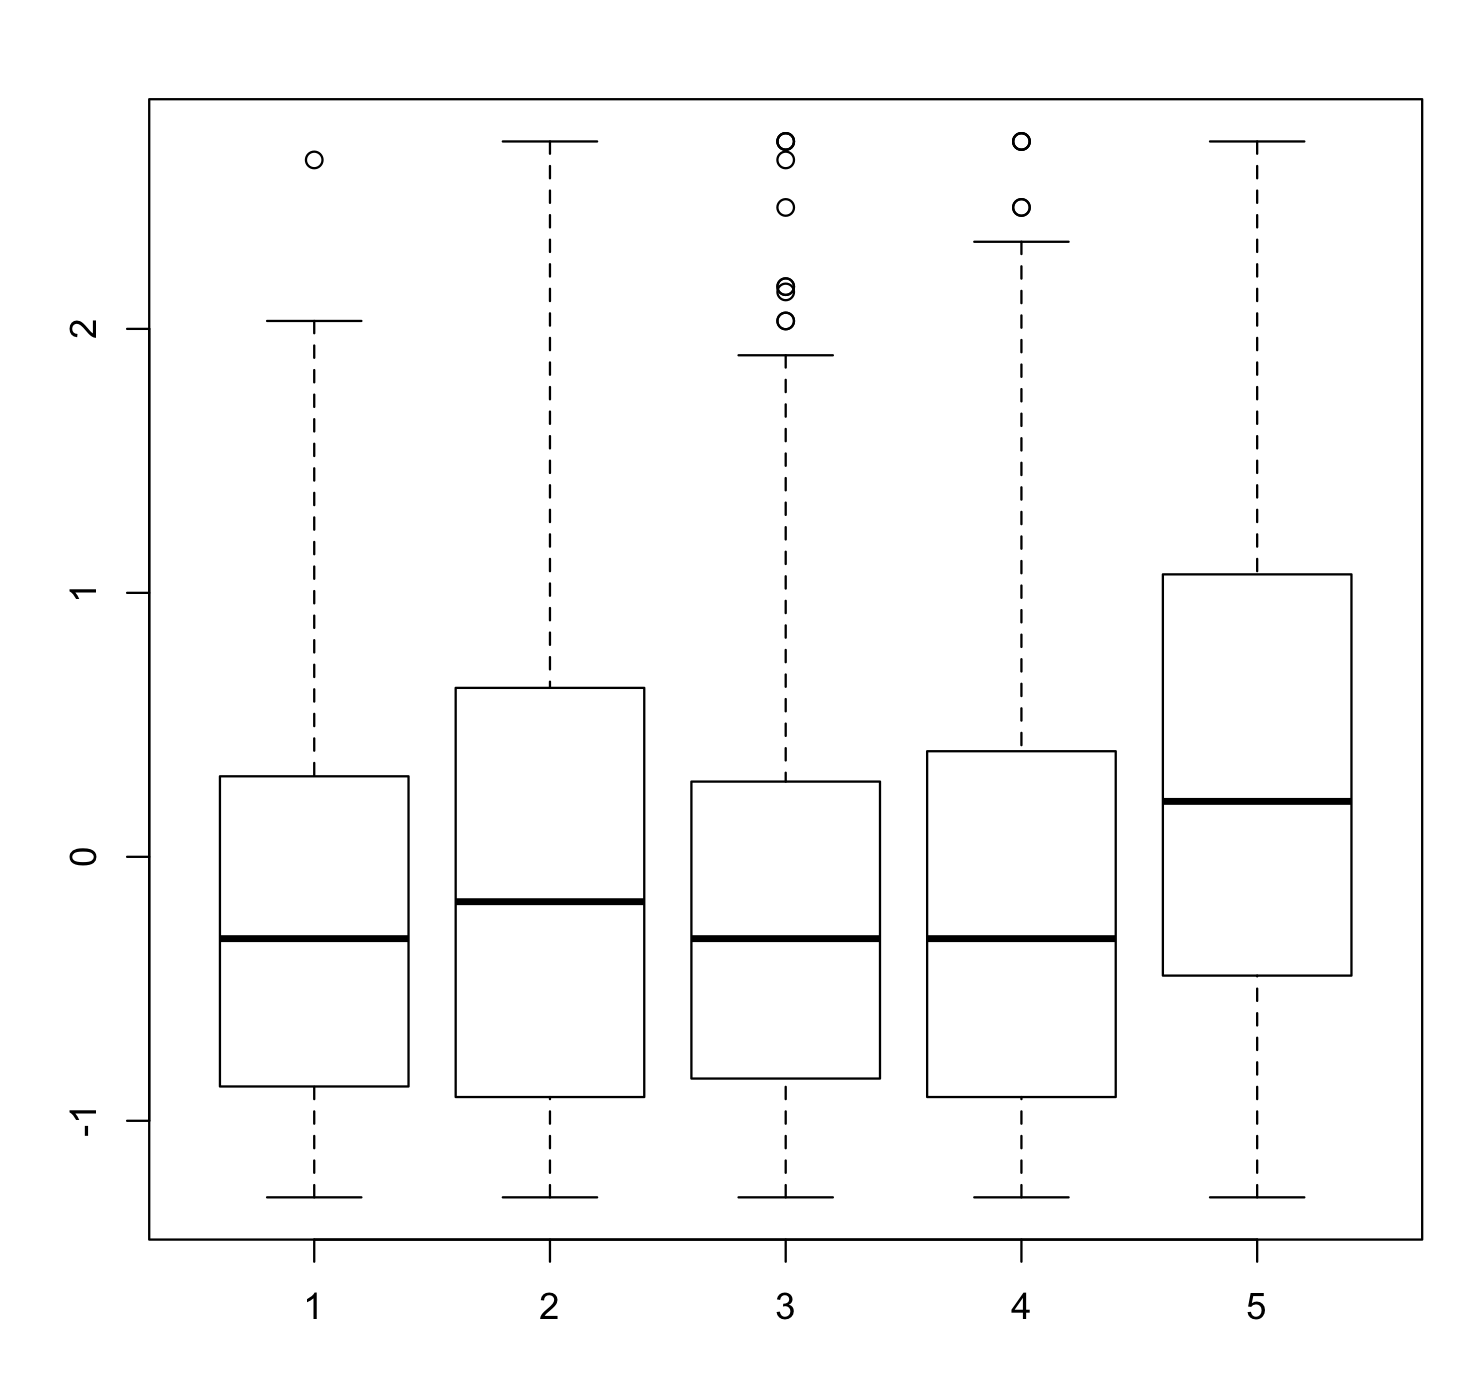
\includegraphics[width=0.8\textwidth]{boxplots}
      \end{figure}

      One selected extract \blockquote{As they pay income taxes} scored particularly poorly with a score of mean score of 2.2/5. Generally ratings correlate with the extract quality. These results are based on 1587 responses for 18 different clusters of extracts from six topics. The target population of this sample is all clusters of extracts selected for display in summaries.

      Regarding the results of the bigram vs. random summary comparison, there appeared was a preference for the bigram summary. 43\% of participants preferred the bigram summary, 20\% scored them the same and 34\% preferred the randomly generated summaries. Breaking this down by topic, the abortion bigram summary scored more than 5 times the random summary; for creation and healthcare both summaries scored equally. Interestingly, the random god summary scored higher than the accompanying bigram one.

      To test these results against \textbf{H3} we again used a one-sided Sign test. Excluding neutral ratings, the bigram model was successful 24/44 times. Based on this result we are unable to reject \textbf{H4}.

    \subsection{\textcolor{red}{TBD: Study 3: Section Comparison}}

  \section{Discussion}
    From our results it is clear that both plain \& layout, point-extract based summaries were significantly preferred overall. However, it is not possible to state with any certainty that formatted are preferred over layout summaries. We are also unable to conclude that the bigram model for extract selection is better than random selection.

    \subsection{Plain vs Stock}
      In the first study, plain summaries were significantly preferred over stock summaries. Participants comments made reference the comparison factors and comments align with score allocated for these. Comparisons that were not captured by the factor ratings were also interesting. Multiple comments made reference to the following comparisons: plain summaries have fewer questions, less surplus information and more content. Comments also made reference to plain summaries being well written with \blockquote{proper English} and \blockquote{complete sentences}. This is particularly interesting considering the point extraction process.

      There were also five comments that suggest the participant believed the summaries to have been written by a human. For example: \blockquote{As I read [STOCK] I felt that I knew the opinion of the writer. With [PLAIN] I could not tell.} and \blockquote{\dots clearer where the author is coming from}. References were also made to higher level properties of the summaries such as \blockquote{logical flow}, \blockquote{relies on fallacy}, \blockquote{explains the reasoning} as well as factual correctness.

      In summary, based on their comments, participants acknowledge succinctness, variety and informativeness even without the explanations and structure of the layout summaries.

    ------

    Based on on comments left as justification, some found the colors distracting and unnecessary as well as making the summary noisy and hard to read.
    Also need some samples of the comments that highlight interesting things

    On average, extracts scored well, showing pre-filtering is good at it's job.

    "Side [RANDOM] uses the scientific method and doesn't involve a fake diety at all in the science section." why god rand was better (also sentences made more sense)
